\chapter{Ergebnis}
Das Ergebnis unseres erfolgreich abgeschlossenen Projekts setzt sich aus zwei Komponenten zusammen:
\begin{itemize}
	\item Untersuchungsbericht
	\item Prototyp
\end{itemize}
\begin{figure}[H]
\centering
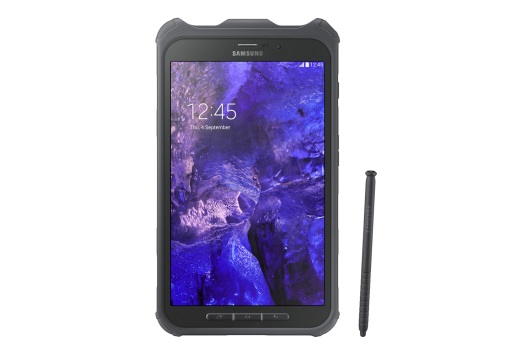
\includegraphics[scale=1.0]{Images/prototyp}
\caption{Der Prototyp}
\end{figure}
Die genauere Definition dieser zwei Komponenten findet man einerseits im Lastenheft, welches wir von unserem Auftraggeber erhalten haben, und andererseits in den von uns vorbereiteten und mit Kapsch abgesprochenen Kriterien, welche in unserem Pflichtenheft abgeklärt wurden. 
\paragraph*{}
Um das Projekt als erfolgreich zu bezeichnen, muss im angesprochenen Untersuchungsbericht ein Vergleich von drei bis vier Softwarelösungen zur Absicherung von Tablets angestellt werden. Zusätzlich müssen zu den jeweiligen Softwarelösungen die diversen Vor– und Nachteile angegeben sein, sowie auch das Fehlen von Einstellungsmöglichkeiten.
\paragraph*{}
Am Ende des Untersuchungsberichts hat ein Vergleich der Systeme zu stehen, aus dem herausgeht, welches, nach der Meinung des Projektteams, eingesetzt werden sollte. Dies muss mit Argumenten bekräftigt werden.
\paragraph*{}
Weiters muss auch der angesprochene Prototyp erstellt bzw. konfiguriert werden. Dieser ist als ein Android–Tablet definiert, welches auf  die Anforderungen eines Beispielunternehmens zugeschnitten ist. Dabei sollen bereits einige Einschränkungen mit der von uns ausgewählten Softwarelösung gemacht worden sein.
\paragraph*{}
Zu diesen Einschränkungen zählt beispielsweise, dass man genau drei bestimmte, vom Auftraggeber festgelegte Apps verwenden darf, dass der Zugang zu den Einstellungen blockiert wird, was bedeutet, dass der User mit dem Tablet nicht in die Einstellungen gehen kann und dort diverse Veränderungen vornehmen kann.
\paragraph*{}
Weiters darf keine Verbindung mit einem Computer im physischen Sinn möglich sein, was bedeutet, dass, falls man das Tablet mit einem Micro USB Kabel an einen Computer anschließt, dieses nicht vom PC erkannt wird und es so nicht verwendet werden kann.
\paragraph*{}
Eine weitere Einschränkung ist, dass man mit dem Tablet keine Apps, Fotos, Videos usw. downloaden können darf.
\paragraph*{}
Die letzte gröbere Einschränkung ist, dass man die gesicherte Umgebung nicht verlassen kann, was bedeutet, dass man die Schutzsoftware nicht ausschalten und das Tablet für seinen privaten Gebrauch verwenden kann.
\paragraph*{}
Sollten diese Kriterien sowohl von unserem Prototypen, als auch von unserem Untersuchungsbericht erfüllt und von Kapsch akzeptiert werden, so erhält dieses Projekt den Status „ERFOLGREICH ABGESCHLOSSEN!“. 